\chapter{Appendix}
\section{Nomenclature}

% ---------- General indices & counts ----------
\begin{table}[H]
    \centering
    \small
    \begin{tabular}{ll}
        \textbf{Symbol} & \textbf{Meaning} \\
        \hline
        $N$ & Number of samples in the (filtered) original dataset $D$ \\
        $i, j$ & Sample indices, $i$ for (para-/model-generated) query, $j$ for original candidate \\
        $a$ & Training iteration index \\
        $l \in \{0,\dots,L\}$ & Layer index (0-based) \\
        $k \in \{0,\dots,K_l\}$ & Component index within layer $l$ \\
        $b$ & Size of the BM25 candidate set $\mathcal{C}_i(b)$ \\
        $P=N\cdot b$ & \#pairs (paraphrased $\times$ BM25 candidates) used in evaluation \\
        \hline
        $\theta$ & Model parameters \\
        $\theta_0$ & Model parameters at the start of training \\
        $\theta_a$ & Model parameters at iteration $a$ \\
        $\theta_T$ & Model parameters at the end of training (fine-tuned model) \\
        $\eta_a$ & Learning rate at iteration $a$ \\
    \end{tabular}
    \caption{General indices and counts.}
    \label{tab:nomenclature-general}
\end{table}

% ---------- Datasets, samples, tokens ----------
\begin{table}[H]
    \centering
    \small
    \begin{tabular}{ll}
        \textbf{Symbol} & \textbf{Meaning} \\
        \hline
        $D=\{s_i\}_{i=0}^{N}$ & Original dataset (instruction–response pairs) \\
        $D_p=\{s_{p_i}\}_{i=0}^{N}$ & Paraphrased dataset (prompt and response paraphrased) \\
        $D_m=\{s_{m_i}\}_{i=0}^{N}$ & Model-generated dataset (paraphrased prompts, model outputs) \\
        $s_i=(s_{i_P}, s_{i_G})$ & Sample $i$: prompt $s_{i_P}$ and generation $s_{i_G}$ \\
        $s_{i_P}=s_i^{-P_i},\dots,s_i^{-1}$ & Prompt tokens of length $P_i$ \\
        $s_{i_G}=s_i^{0},\dots,s_i^{G_i}$ & Generation tokens of length $G_i$ \\
        $s_{p_i}=(s_{p_{i_P}}, s_{p_{i_G}})$ & Paraphrased sample \\
        $s_{m_i}=(s_{m_{i_P}}, s_{m_{i_G}})$ & Model-generated sample ($s_{m_{i_P}}=s_{p_{i_P}}$) \\
        $\operatorname{LLM}_{\text{para}}(\cdot)$ & Paraphrasing model/function \\
        $\operatorname{LLM}(\cdot)$ & Model under evaluation (produces $s_{m_{i_G}}$) \\
    \end{tabular}
    \caption{Datasets, samples, and tokenization.}
    \label{tab:nomenclature-data}
\end{table}

% ---------- Loss & training ----------
\begin{table}[H]
    \centering
    \small
    \begin{tabular}{ll}
        \textbf{Symbol} & \textbf{Meaning} \\
        \hline
        $\mathcal{L}(s_i^j,\theta)$ & Token-level loss at token $j$ of sample $i$ \\
        $\mathcal{L}(s_i,\theta)=\frac{1}{G_i}\sum_{j=0}^{G_i}\mathcal{L}(s_i^j,\theta)$ & Per-sample loss \\
        $p_\theta(s_i^j \mid s_i^{-P_i},\dots,s_i^{j-1})$ & Next-token probability under the model \\
        $\nabla_{\theta}\mathcal{L}(s_i,\theta)$ & Gradient of loss w.r.t.\ $\theta$ for sample $s_i$ \\
        $\theta_{a+1}=\theta_a-\eta_a\nabla_{\theta}\mathcal{L}(s_a,\theta_a)$ & Gradient descent update \\
    \end{tabular}
    \caption{Loss and training notation.}
    \label{tab:nomenclature-loss}
\end{table}

% ---------- Architecture & parameters ----------
\begin{table}[H]
    \centering
    \small
    \begin{tabular}{ll}
        \textbf{Symbol} & \textbf{Meaning} \\
        \hline
        $\mathcal{W}=\{(l,k)\}$ & Index set of all layer components \\
        $\mathbf{W}^{(l,k)}$ & Parameter matrix of component $k$ in layer $l$ \\
        $L$ & Number of decoder layers \\
        $K_l$ & Number of components in layer $l$ \\
        $M$ & Total trainable parameters \\
        $\mathbf{E}\in\mathbb{R}^{|V|\times d_x}$ & Input embedding matrix \\
        $\mathbf{W}^{(o)}=\mathbf{E}^{\top}\in\mathbb{R}^{d_x\times|V|}$ & Tied LM head (output projection) \\
        $|V|$ & Vocabulary size \\
        $d_x$ & Hidden size \\
        $d_{ff}$ & Feed-forward (MLP) width \\
        $\mathbf{W}^{(l)}_{\mathrm{Q}},\mathbf{W}^{(l)}_{\mathrm{K}},\mathbf{W}^{(l)}_{\mathrm{V}},\mathbf{W}^{(l)}_{\mathrm{O}}$ & Attention Q/K/V/O projections in layer $l$ \\
        $\mathbf{W}^{(l)}_{\text{gate}},\mathbf{W}^{(l)}_{\text{up}},\mathbf{W}^{(l)}_{\text{down}}$ & MLP gate/up/down projections in layer $l$ \\
        $M_H$ & Naive param count without weight-tying \\
        $\Delta_M$ & Difference due to tying ($\Delta_M=|V|\cdot d_x$ here) \\
    \end{tabular}
    \caption{Model/parameter notation.}
    \label{tab:nomenclature-params}
\end{table}

% ---------- Operators & gradient flattening ----------
\begin{table}[H]
    \centering
    \small
    \begin{tabular}{ll}
        \textbf{Symbol} & \textbf{Meaning} \\
        \hline
        $\operatorname{vec}_r(\cdot)$ & Row-major vectorization $\mathbb{R}^{m\times n}\!\to\!\mathbb{R}^{mn}$ \\
        $\operatorname{col}(x_1,\dots,x_m)$ & Collector/concatenation: stack vectors vertically \\
        $\odot,\ \oslash$ & Elementwise product and elementwise division \\
        $\mathbf{v}_{\mathbf{W}^{(l,k)}}(s_i)=\operatorname{vec}_r\big(\nabla_{\mathbf{W}^{(l,k)}}\mathcal{L}(s_i,\theta_T)\big)$ & Flattened gradient for component $(l,k)$ \\
        $\mathbf{v}_{\theta}(s_i)=\operatorname{col}\big(\mathbf{v}_{\mathbf{W}^{(0,0)}}(s_i),\dots,\mathbf{v}_{\mathbf{W}^{(L,K_L)}}(s_i)\big)$ & Full flattened gradient for $s_i$ \\
        $\mathbf{v}_{\bullet}(s_i)$, $\mathbf{v}_{\bullet}[\mathcal{S}]$ & Same, restricted to a component or a set $\mathcal{S}\subseteq\mathcal{W}$ \\
    \end{tabular}
    \caption{Operators and flattened gradient vectors.}
    \label{tab:nomenclature-ops}
\end{table}

% ---------- Similarities & scores ----------
\begin{table}[H]
    \centering
    \small
    \begin{tabular}{ll}
        \textbf{Symbol} & \textbf{Meaning} \\
        \hline
        $\langle \mathbf{a},\mathbf{b}\rangle=\mathbf{a}^{\top}\mathbf{b}$ & Dot product \\
        $\simcos(\mathbf{a},\mathbf{b})=\dfrac{\mathbf{a}^{\top}\mathbf{b}}{\|\mathbf{a}\|\,\|\mathbf{b}\|}$ & Cosine similarity \\
        $\gamma_{i,j}^{\theta}=\simcos\big(\mathbf{v}_{\theta}(\,s_{p_i}\,),\mathbf{v}_{\theta}(\,s_{j}\,)\big)$ & Full-model similarity (paraphrased $\to$ original) \\
        $\Gamma^\theta\in\mathbb{R}^{P}$ & Vector stacking all $\gamma_{i,j}^{\theta}$ over evaluated pairs \\
        $\delta^{(l,k)}_{i,j}$ & Per-component cross dot: $\mathbf{v}_{\mathbf{W}^{(l,k)}}(s_{p_i})^{\top}\mathbf{v}_{\mathbf{W}^{(l,k)}}(s_j)$ \\
        $\delta^{(l,k)}_{i,i},\,\delta^{(l,k)}_{j,j}$ & Per-component self-dots for $s_{p_i}$ and $s_j$ \\
        $D^{\mathcal{L}}_{i,j}$ & Accumulated cross dot over $\mathcal{L}$: $\sum_{(l,k)\in\mathcal{L}}\delta^{(l,k)}_{i,j}$ \\
        $\hat{\gamma}^{\mathcal{L}}_{i,j}=\dfrac{D^{\mathcal{L}}_{i,j}}{\sqrt{D^{\mathcal{L}}_{i,i}}\sqrt{D^{\mathcal{L}}_{j,j}}}$ & Reconstructed cosine from selected components \\
        $\hat{\Gamma}^{\mathcal{L}}$ & Vector stacking all $\hat{\gamma}^{\mathcal{L}}_{i,j}$ \\
        $\rho(\mathcal{L})=\simcos\big(\hat{\Gamma}^{\mathcal{L}},\Gamma^\theta\big)$ & Agreement with full-model similarities \\
    \end{tabular}
    \caption{Similarities, dot-product caches, and reconstructed scores.}
    \label{tab:nomenclature-sims}
\end{table}

% ---------- Candidate selection & metrics ----------
\begin{table}[H]
    \centering
    \small
    \begin{tabular}{ll}
        \textbf{Symbol} & \textbf{Meaning} \\
        \hline
        $\operatorname{BM25}_D(s_{p_i}, s_j)$ & BM25 score of $s_j$ for query $s_{p_i}$ over corpus $D$ \\
        $\mathcal{C}_i(b)$ & Ordered index set of top-$b$ BM25 candidates for $s_{p_i}$ (contains $i$) \\
        $\operatorname{accuracy}_{\theta}(D_p,D)$ & Top-1 retrieval accuracy using full gradients over all $j$ \\
        $\operatorname{accuracy}^{(b)}_{\theta}(D_p,D)$ & BM25-restricted accuracy (compare only $j\in\mathcal{C}_i(b)$) \\
        $\operatorname{accuracy}^{(b)}_{\mathbf{W}^{(l,k)}}(D_p,D)$ & Per-component accuracy (using $\mathbf{v}_{\mathbf{W}^{(l,k)}}$) \\
        $\operatorname{accuracy}^{(b)}_{\mathcal{L}}(D_p,D)$ & Accuracy using the selected set $\mathcal{L}$ \\
        $\varepsilon$ & Small constant for numerical stability in divisions \\
    \end{tabular}
    \caption{Candidate selection (BM25) and retrieval metrics.}
    \label{tab:nomenclature-bm25-metrics}
\end{table}

% ---------- Greedy layer selection ----------
\begin{table}[H]
    \centering
    \small
    \begin{tabular}{ll}
        \textbf{Symbol} & \textbf{Meaning} \\
        \hline
        $\mathcal{L}$ & Set of selected layer components (grows during forward greedy) \\
        $\mathcal{R}=\mathcal{W}\setminus\mathcal{L}$ & Remaining components not yet selected \\
        $((l_t,k_t),\,\rho_t)$ & $t$-th selected component and running similarity score \\
        $((l_t,k_t),\,a_t)$ & $t$-th selected component and running accuracy score \\
    \end{tabular}
    \caption{Greedy forward layer selection notation.}
    \label{tab:nomenclature-greedy}
\end{table}

% ---------- Random projection baseline ----------
\begin{table}[H]
    \centering
    \small
    \begin{tabular}{ll}
        \textbf{Symbol} & \textbf{Meaning} \\
        \hline
        $\mathbf{R}\in\mathbb{R}^{d\times M}$ & Random projection matrix (Rademacher) for full vector (conceptual) \\
        $\mathbf{R}^{(l,k)}\in\mathbb{R}^{d_{(l,k)}\times |\mathbf{W}^{(l,k)}|}$ & Per-component projector (used in practice) \\
        $d,\ d_{(l,k)}$ & Projection dimensions (global / per component) \\
        $d_{\text{proj}}$ & Target total projection dimension (budget) \\
        $d_{\min}$, $g$ & Min per-component dim and rounding granularity \\
        $P_{(l,k)}$ & Parameter count of component $(l,k)$ \\
        $\mathbf{p}(s_i)$ & Concatenated projected gradient for sample $s_i$ \\
    \end{tabular}
    \caption{Random projection baseline notation.}
    \label{tab:nomenclature-rp}
\end{table}


\section{AMD-OLMo-1B-SFT}
The number of parameters as a horizontal bar graph is shown in Figure~\ref{fig:parameters_per_layer_amd_olmo}.
\begin{figure}[ht]
    \centering
    
\includegraphics[width=0.63\textwidth]{figures/parameters_per_layer.png}
    \caption{Visual representation of the parameters per layer component for model \texttt{AMD-OLMo-1B-SFT} on a logarithmic scale.}
    \label{fig:parameters_per_layer_amd_olmo}
\end{figure}

\section{Preliminary Analysis of Gradient Dot Products}
A preliminary analysis of gradient dot products between $25$ paraphrased and original samples is shown in Figure~\ref{fig:preliminary_analysis_dot_products}. As illustrated there, the main diagonal contains significantly higher values, indicating that the model is able to find the corresponding original data points. 

\begin{figure}[ht]
    \centering
    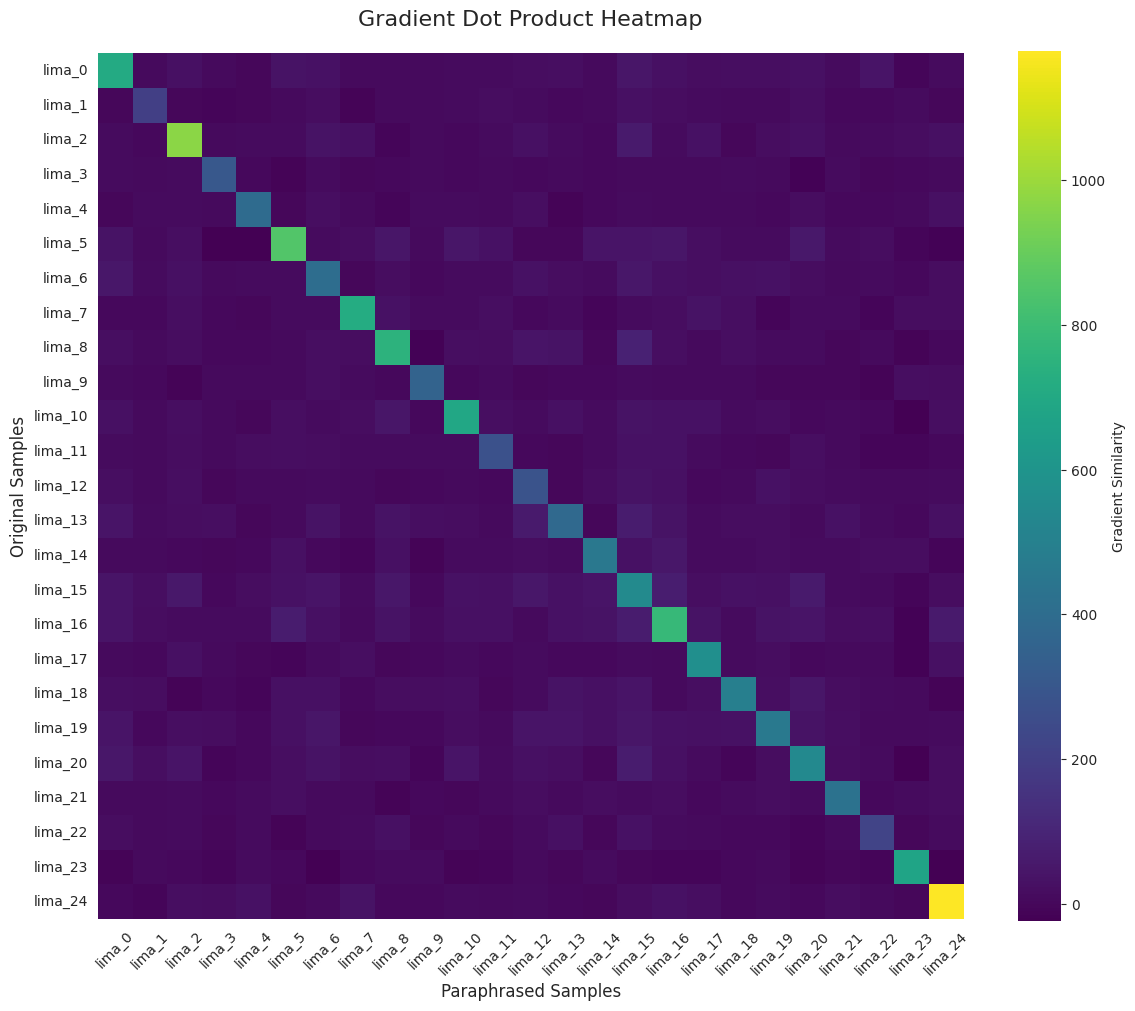
\includegraphics[width=1\textwidth]{figures/preliminary_analysis_dot_products.png}
    \caption{Preliminary analysis of gradient dot products between paraphrased and original samples.}
    \label{fig:preliminary_analysis_dot_products}
\end{figure}

\section{Dataset Examples}

\subsection{Paraphrased}\label{subsec:appendix_paraphrased_sample}
The paraphrased equivalent for the presented example for the \emph{LIMA} dataset illustrated in Subsection~\ref{subsec:lima_dataset}.
\\\\
Paraphrased user message $s_{p_{0_P}}$:
\begin{verbatim}
    Are brain cells capable of moving? Specifically, I'm referring to 
    long-distance migration, ideally occurring within the brain.
\end{verbatim}
Paraphrased assistant message $s_{p_{0_G}}$:
\begin{verbatim}
    The inquiry is quite extensive, and it’s important to recognize that the
    brain is made up not only of neurons but also of glial cells (supporting 
    cells) and pre-mitotic neuronal stem cells. Additionally, as critical 
    colleagues in research have pointed out, the developmental stage is 
    crucial, since the developing embryonic brain is significantly different 
    from the fully developed adult brain. Nonetheless, after reviewing various 
    studies, the answer to the question turns out to be surprisingly 
    straightforward: Yes, brain cells do migrate. In the adult brain, glial 
    cells are known to migrate (Klämbt, 2009). These glial cells perform 
    numerous functions, with a prominent example being oligodendrocytes, 
    which migrate over considerable distances to locate their target axons 
    and encase them to create the insulating myelin sheath 
    (Tsai and Miller, 2002). Neuronal stem cells also migrate long distances
    in response to injury (Imitola et al., 2004), moving from specific 
    stem-cell areas (such as the hippocampus and subventricular zone) to 
    other parts of the brain (Clarke, 2003). It has been demonstrated that 
    post-mitotic but non-differentiated neurons can migrate within the 
    adult brain in fish (Scott et al., 2012) and also in mammals and 
    non-human primates (Sawada et al., 2011). Unsurprisingly, glial cells, 
    stem cells, and neurons also undergo migration during embryonic 
    development. Most notably, post-mitotic neurons that are intended for 
    peripheral roles must migrate over relatively long distances from the 
    neural crest to their designated target areas 
    (Neuroscience, 2nd ed, Neuronal Migration).
\end{verbatim}

\subsection{Model-Generated}\label{subsec:appendix_model_generated_sample}
The model-generated equivalent for the presented example for the \emph{LIMA} dataset illustrated in Subsection~\ref{subsec:lima_dataset}.
\\\\
Model-generated user message $s_{p_{0_P}} = s_{m_{0_P}}$:
\begin{verbatim}
    Are brain cells capable of moving? Specifically, I'm referring to
    long-distance migration, ideally occurring within the brain.
\end{verbatim}
Model-generated assistant message $s_{m_{0_G}}$:
\begin{verbatim}
    Brain cells, such as neurons, are indeed capable of moving. This 
    movement is crucial for various functions, including communication 
    between neurons and the formation of neural networks. However, the 
    extent of brain cell movement is limited by the physical constraints
    of the brain's structure.

    Neurons are highly organized and interconnected, forming complex 
    networks that enable the brain to process and interpret information.
    The movement of neurons within these networks is facilitated by the 
    cytoskeleton, which provides structural support and allows for the 
    movement of the cell body.
    
    While brain cells can move within the brain, the movement is typically
    limited to short distances and is not as extensive as the movement of 
    neurons in other parts of the body. The brain's structure and the 
    limitations of its physical constraints prevent the movement of brain
    cells over long distances.
    ####
    Yes, brain cells can move, but it is limited to short distances within 
    the brain.
\end{verbatim}

\section{Results}

\subsection{Accuracy per Layer Component}

\subsubsection{Paraphrased}
\begin{figure}[ht]
    \centering
    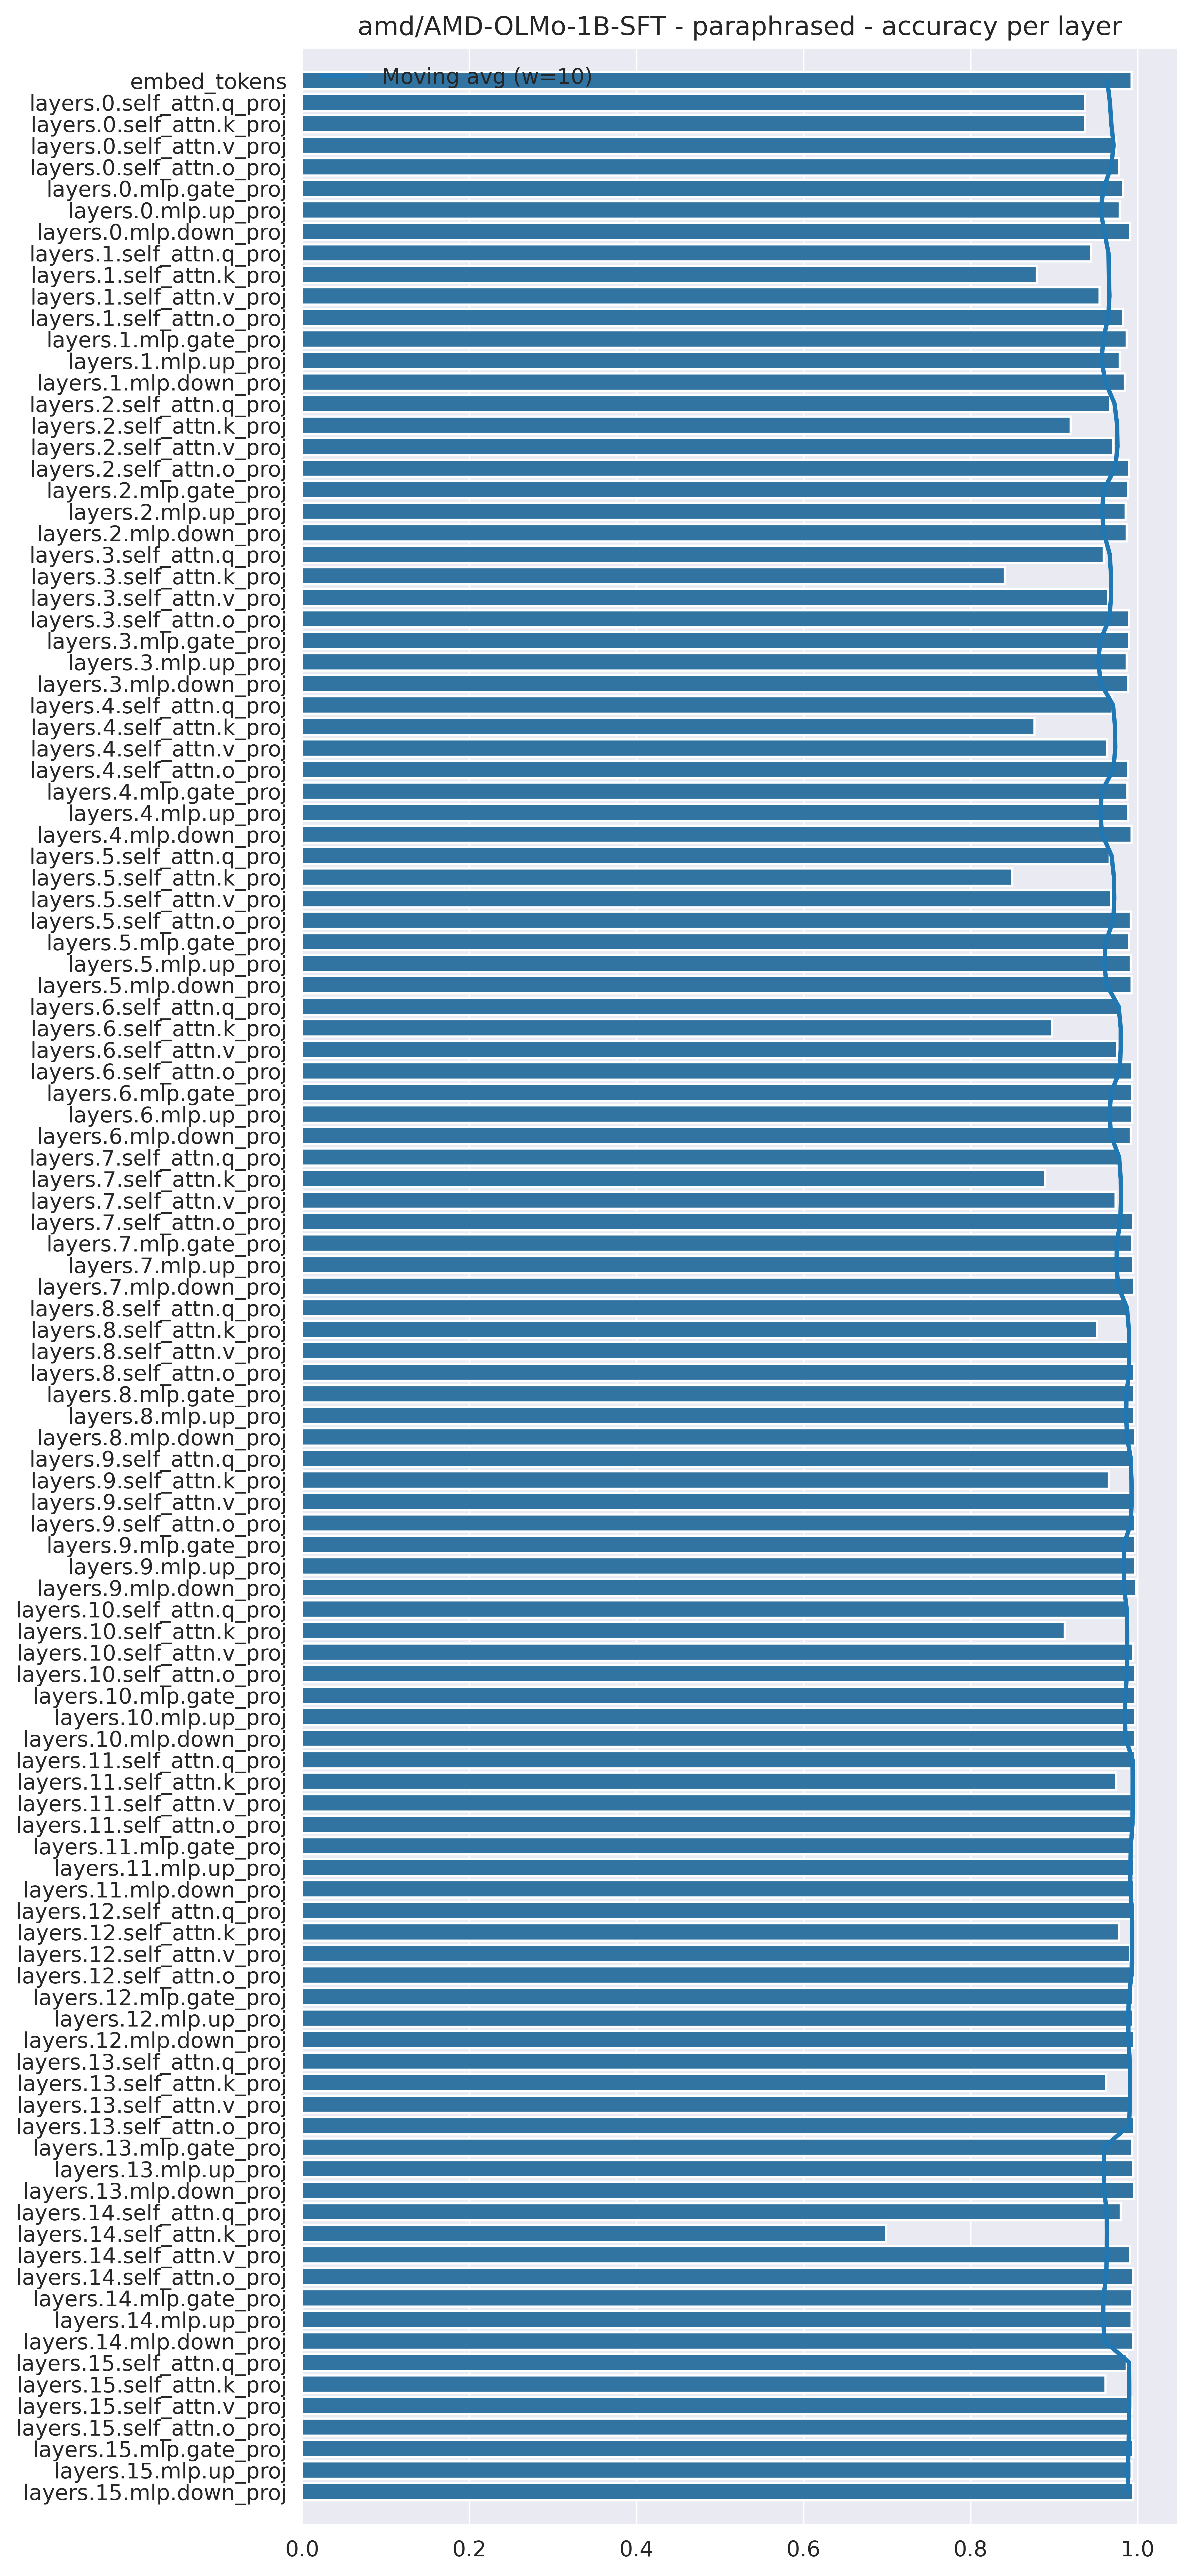
\includegraphics[width=0.63\textwidth]{figures/results/paraphrased/accuracy_per_layer.png}
    \caption{Accuracy per layer in the paraphrased setting}
    \label{fig:paraphrased_accuracy_per_layer}
\end{figure}

\subsubsection{Model-generated}
\begin{figure}[ht]
    \centering
    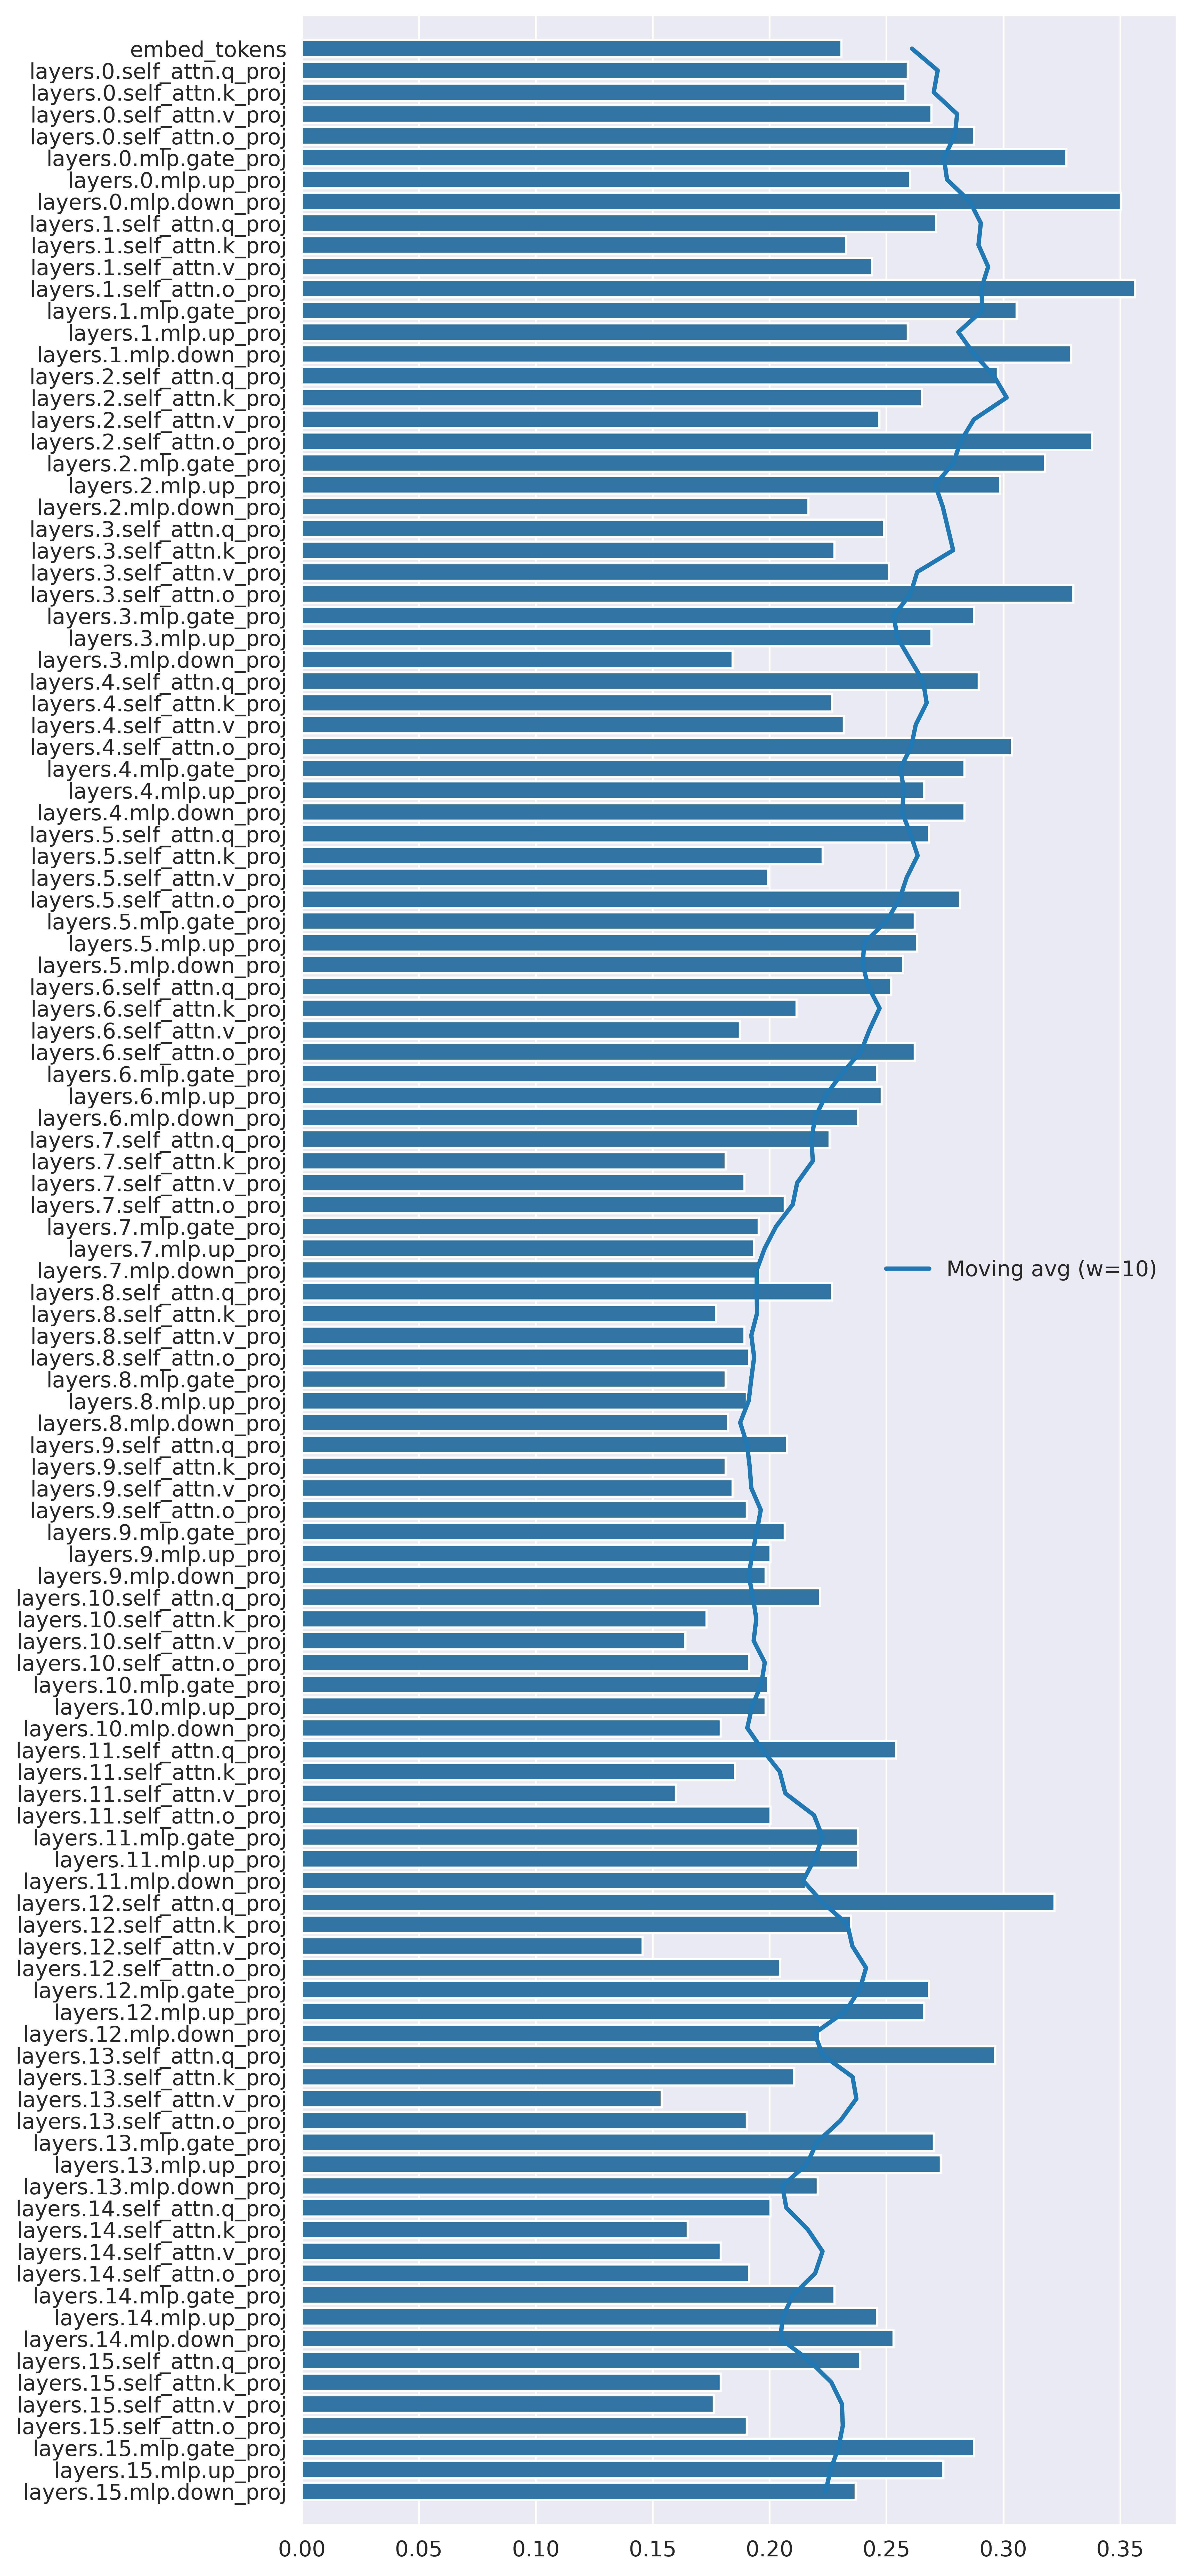
\includegraphics[width=0.63\textwidth]{figures/results/model-generated/accuracy_per_layer.png}
    \caption{Accuracy per layer in the model-generated setting}
    \label{fig:model_generated_accuracy_per_layer}
\end{figure}

\subsection{Comparison between Layer Components and Full Gradient}

\subsubsection{Paraphrased}
\begin{figure}[ht]
    \centering
    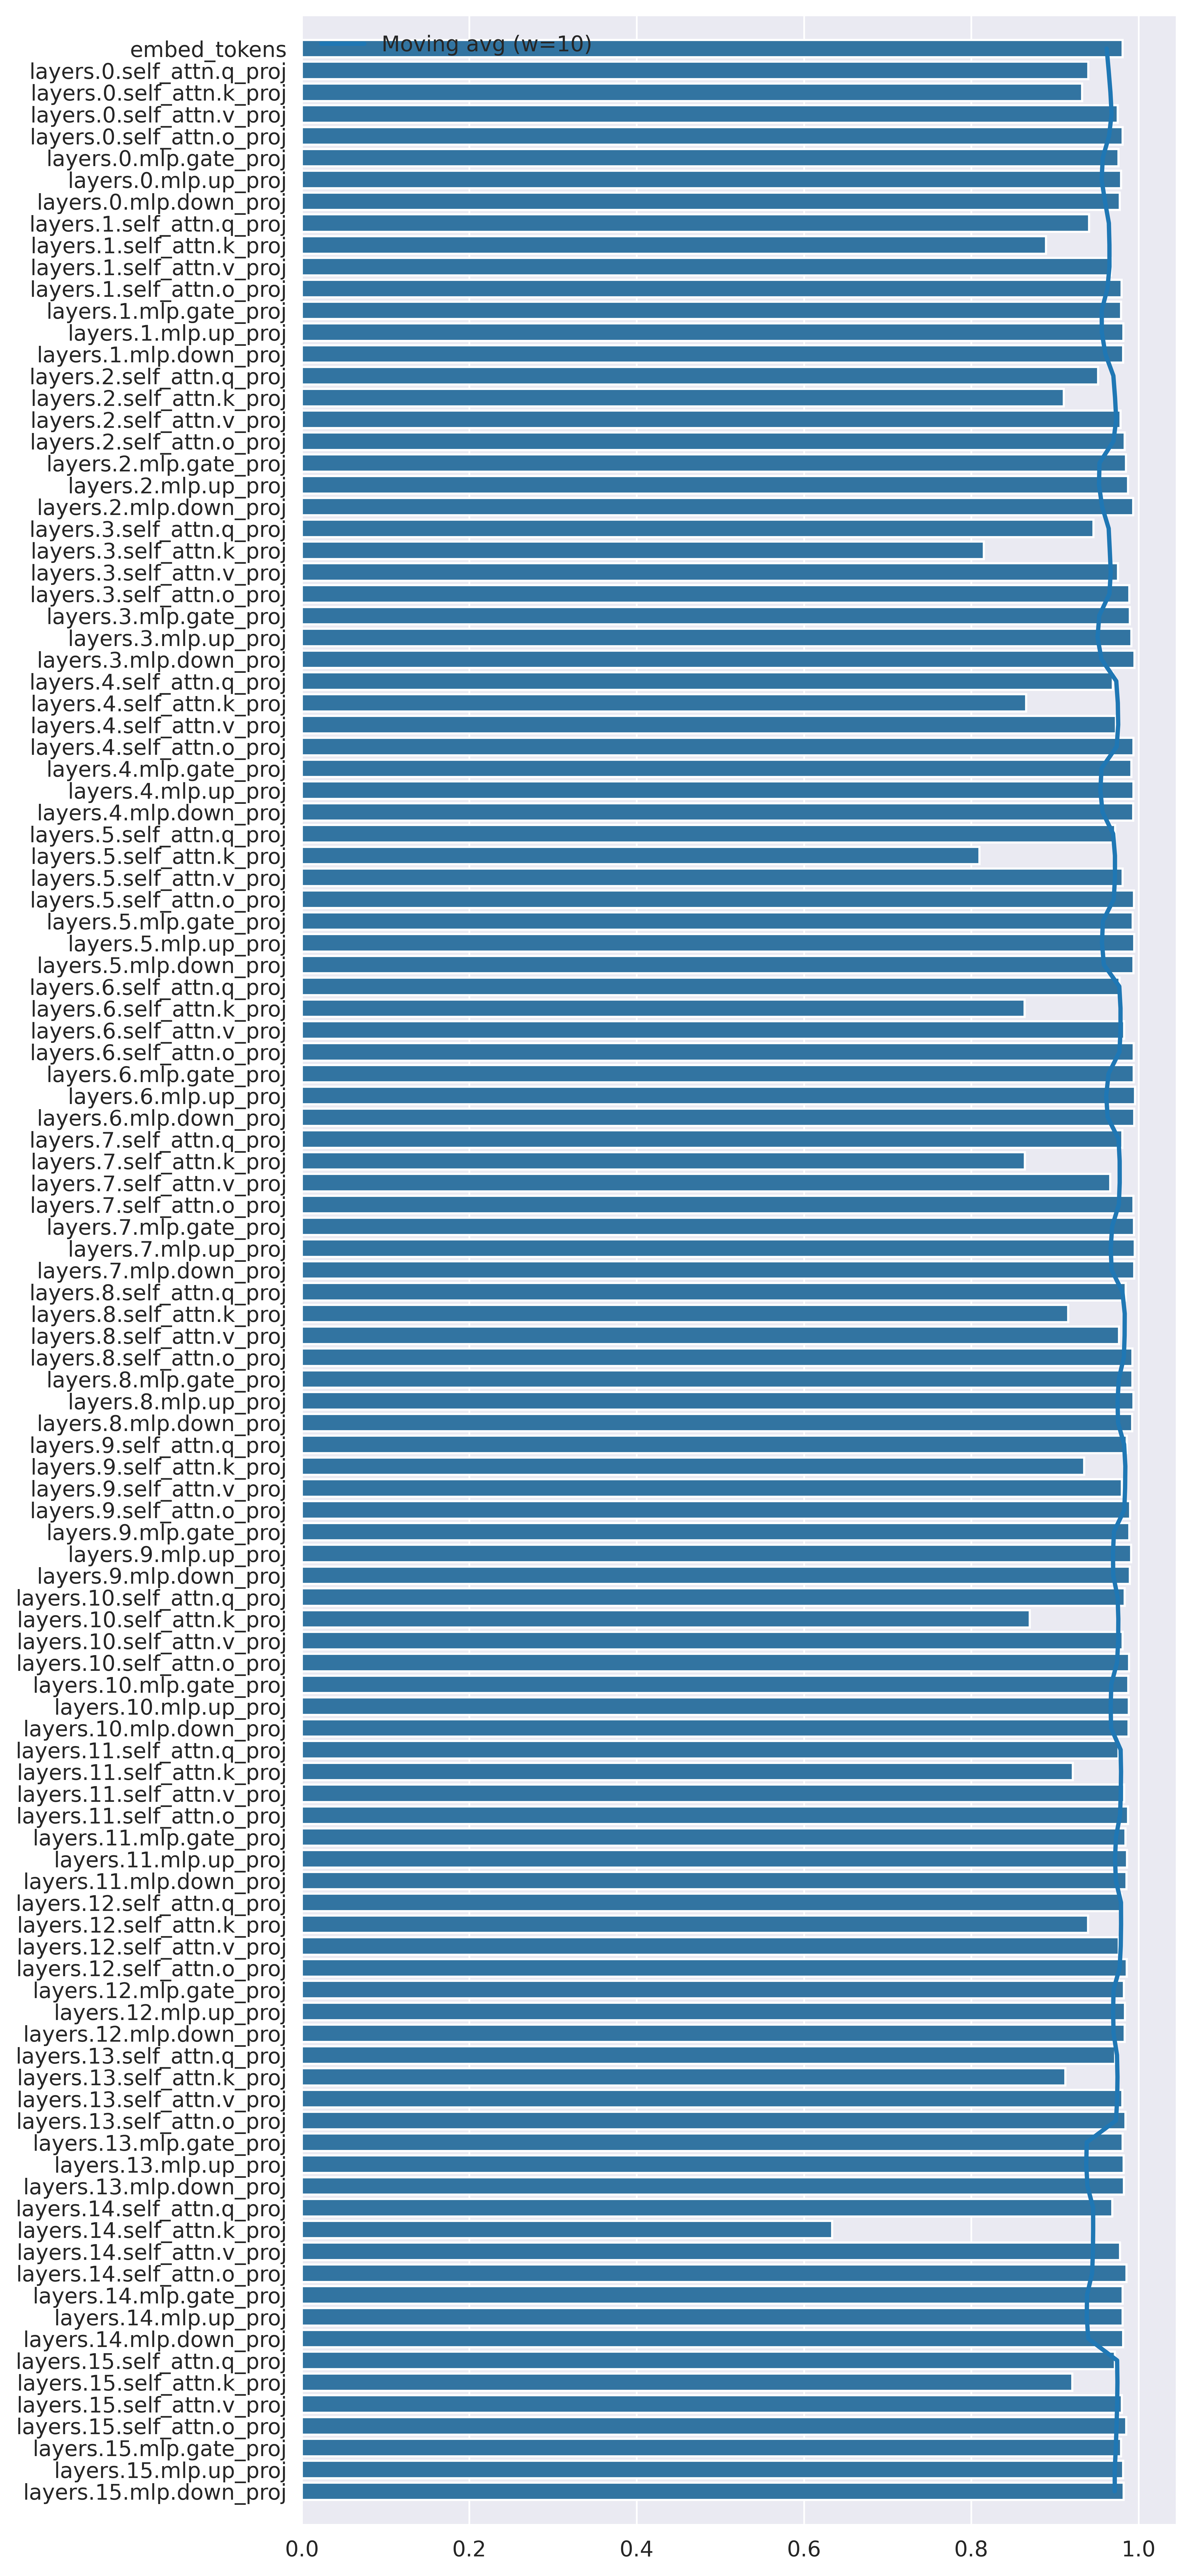
\includegraphics[width=0.63\textwidth]{figures/results/paraphrased/layer_comparison_full_gradient.png}
    \caption{Comparison of single layer component and full model gradient scores for the paraphrased setting.}
    \label{fig:paraphrased_layer_comparison_full_gradient}
\end{figure}

\subsubsection{Model-generated}

\subsubsection{Paraphrased}
\begin{figure}[ht]
    \centering
    \includegraphics[width=0.63\textwidth]{figures/results/model-generated/layer_comparison_full_gradient.png}
    \caption{Comparison of single layer component and full model gradient scores for the model-generated setting.}
    \label{fig:model_generated_layer_comparison_full_gradient}
\end{figure}

\section{Code and Repository}
The complete project code can be found on the following GitHub repository: \url{https://github.com/lukas-hinterleitner/master-thesis}.
